%!TEX TS-program = xelatex
%!TEX encoding = UTF-8 Unicode
Se utilizó el algoritmo \textbf{AgglomerativeClustering} de la librería sklearn extra.cluster y con la métrica de distancia euclidean.

\subsection{Resultados}
\subsubsection{Audio Features}
\begin{center}\textbf{Dendogramas}\end{center}


En un primer analisis, tuvimos que decidir que tipo de distancia utilizariamos para formar los clusters, la funcion AgglomerativeClustering nos daba cuatro opciones de linkage criterion:

\begin{itemize}
  \item \textbf{ward} Minimiza la varianza de los clusters que son mergeados.
  \item \textbf{average} Computa la distancia media de cada observacion de dos conjuntos.
  \item \textbf{single} Usa la maxima distancia entre todas las observaciones de dos conjuntos.
  \item\textbf{complete} Usa la maxima distancia entre todas las observaciones de dos conjuntos.
\end{itemize}

Se generan los 4 dendogramas para estudiar que criterio agrupa mejor los datos.

\begin{figure}[H]
{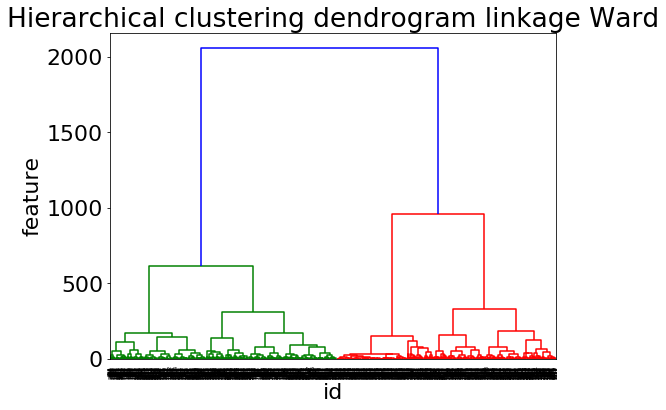
\includegraphics[width = 3in]{img/imagenes/jerarquico_AF/dendongrama_ward.png}} 
{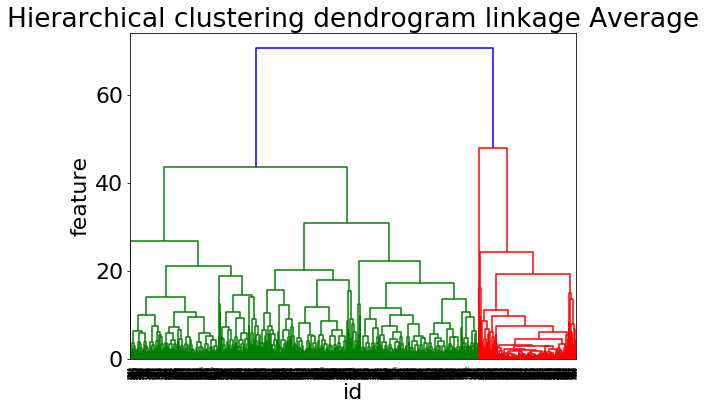
\includegraphics[width = 3in]{img/imagenes/jerarquico_AF/dendongrama_average.png}}\\
{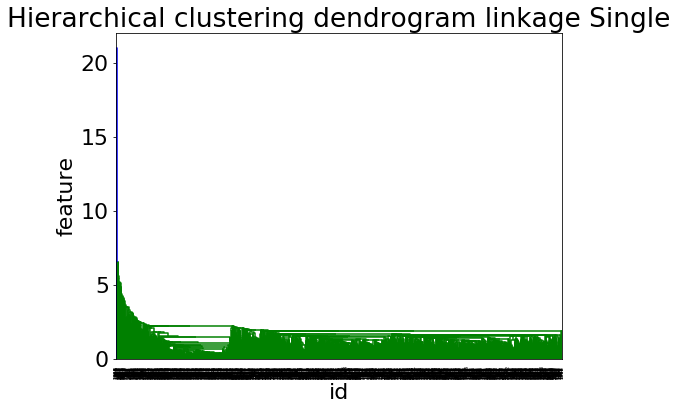
\includegraphics[width = 3in]{img/imagenes/jerarquico_AF/dendongrama_single.png}}
{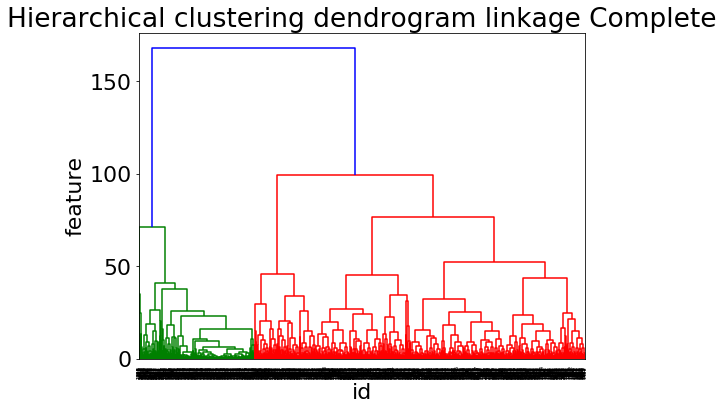
\includegraphics[width = 3in]{img/imagenes/jerarquico_AF/dendongrama_complete.png}} 
\label{Comparativa entre linkage criterions}
\end{figure}

Al revisar la salida de los distintos linkages, lo que podemos observar es que el metodo \textbf{ward} es quien esta manteniendo un mayor balance entre los distintos clusters. Revisando en detalle dicho dendograma, podemos concluir en principio que una separacion natural podria ser en 2, 3 o 4 clusters ya que determinamos que con esta cantidad se podria generar un balanceo entre el tamaño de los mismos.

\begin{figure}[H]
    \centering
    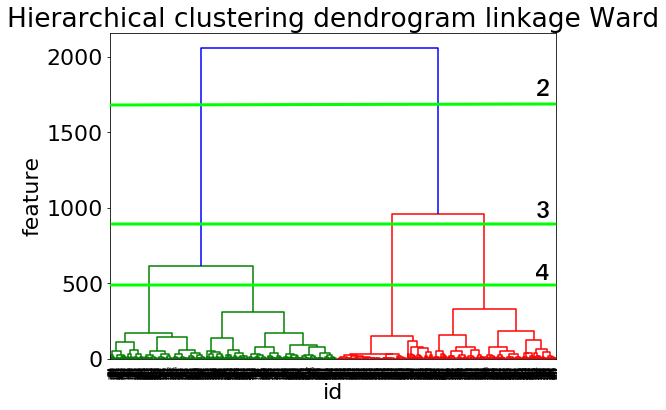
\includegraphics[width=\textwidth]{img/imagenes/jerarquico_AF/dendongrama_ward_clusters.png}
    \caption{Posibles separaciones en Clusters}
    \label{fig:clusters}
\end{figure}

Si bien dicha apreciación podria ser verdadera, nos disponemos a estudiar distintos coeficientes y tecnicas que nos permitiran entender cual es el mejor \textbf{K} para este metodo.

\begin{center} \textbf{Coeficiente de Silhouette} \end{center}
Para determinar en que cantidad de clusters conviene mas realizar la separaciones, nos basamos en el coeficiente de Silhouette, el cual nos da una medida para saber cual es el \textbf{K} óptimo para construir la separación. Se realizó el computo de dicho coeficiente para 2, 3, 4, 5 y 6 divisiones como para tener una imagen mas completa sobre como se estan comportando los datos.

\begin{figure}[H]
    \centering
    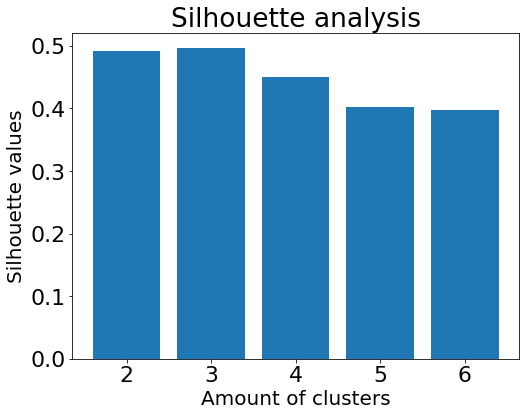
\includegraphics[width=\textwidth]{img/imagenes/jerarquico_AF/silhouette_general.png}
    \label{fig:silGeneral}
\end{figure}

\newpage
Como podemos ver en el resultado, claramente con un \textbf{K=2} o \textbf{K=3} se obtiene el mejor coeficiente, nos disponemos ahora a realizar un analisis un poco mas profundo sobre estos valores para tomar una decision, graficaremos los coeficientes comparando ahora para 2, 3 divisiones. 

\begin{figure}[h]
{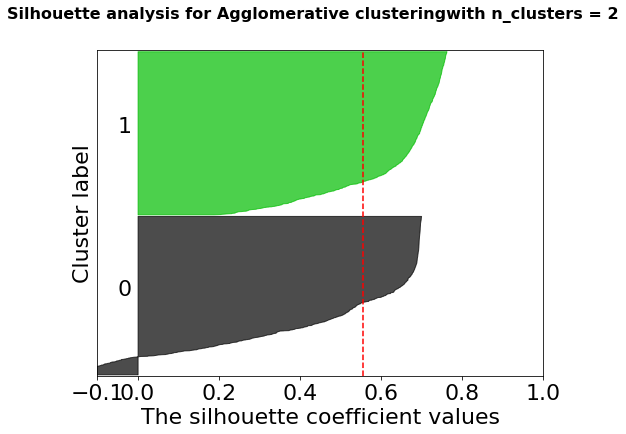
\includegraphics[width = 3in]{img/imagenes/jerarquico_AF/silhouette_2.png}} 
{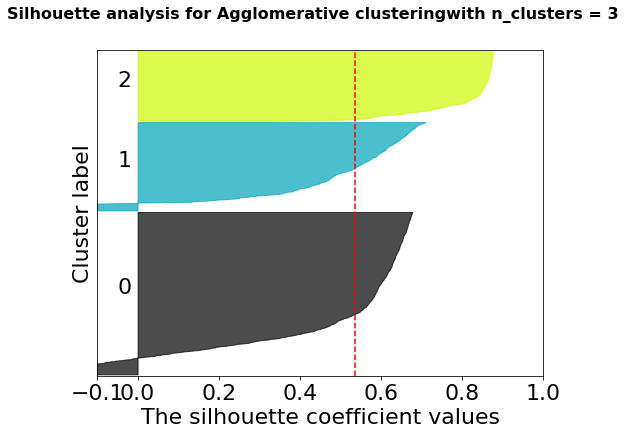
\includegraphics[width = 3in]{img/imagenes/jerarquico_AF/silhouette_3.png}}\\
\label{fig: Comparativa entre Silhouette}
\end{figure}

\begin{table}[H]
    \centering
    \begin{tabular}{|c|c|}
		\hline
        Cantidad de clusters & Silhouette Score \\
        \hline
        2 & 0.5566\\
        3 & 0.5362\\
        \hline
    \end{tabular}
    \caption{Silhouette Score}
    \label{tab:clus-sil}
\end{table}

Si bien se obtiene un mejor coeficiente para un \textbf{K=2}, como la diferencia entre este y el \textbf{K=3} es muy pequeña seleccionaremos al K=3 ya que nos permite contar con mas agrupaciones y poder lograr una separacion en clusters mas interesante.

\begin{center} \textbf{Cross table} \end{center}
Para entender a mas a detalle que tan bien se realizo la clasificaciones se genera la siguiene tabla donde se aprecia el agrupamiento de generos en los dinstios clusters.

\begin{table}[H]
    \centering
    \begin{tabular}{|c|c|c|c|}
        \hline
        & \multicolumn{3}{ c| }{Clusters} \\
        \hline
        Género & 0 & 1 & 2 \\
        \hline
        ambient & 274 & 154 & 32 \\
        classical & 308 & 72 & 25 \\
        drum-and-bass & 42 & 55 & \textbf{354} \\
        jazz & 240 & 153 & 34 \\
        world-music & 255 & 175 & 33 \\   
        \hline
    \end{tabular}
    \caption{Géneros musicales y grupos}
    \label{tab:cross-af}
\end{table}

Podemos observar que el mejor agrupamiento lo tenemos en el cluster 2, con el genero \textbf{drum-and-bass}. Al igual que  con K-means y con PAM dicho genero es quien concentro en un cluster la mayor cantidad de observaciones.
Se dispone a analizarlos índices de RAND y VanDongen para evaluar si los agrupamientos son similares para los distintos conjuntos de datos.

\begin{table}[H]
	\centering
	\begin{tabular}{ |c|c|c| }
		\hline 		
 		Cantidad de clusters & Indice RAND & Indice VanDongen\\ 
 		\hline
 		2 & 0.1918 & 0.7805\\ 
 		3 & 0.3085 & 0.7575\\
 		\hline    
	\end{tabular}
     \label{tab:clus-rand-vand}
\end{table}

Si bien tomamos la decisión de elegi un \textbf{K=3}, algunos analisis los haremos con \textbf{K=2} tambien para comparar en todo momento que nuestra
elección haya sido adecuada.

Con el índice de VanDongen se observa un alto grado de pureza con los clusters analizados, mas de un $75\%$.
Para el índice RAND podemos comentar que el porcentaje de decisiones correctas del cluster es de
$30\%$ sin embargo es de esperable tener un porcentaje bajo ya que se están realizando agrupaciones de 3
clusters a diferencia de las 5 etiquetas de género en los datos.

\begin{center} \textbf{Componentes principales} \end{center}
A continuación se realizó análisis de componentes principales con la finalidad de reducir la dimensionalidad del data set estudiado y
asi poder lograr una representación gráfica de la division en 3 clusters.

\begin{figure}[H]
    \centering
    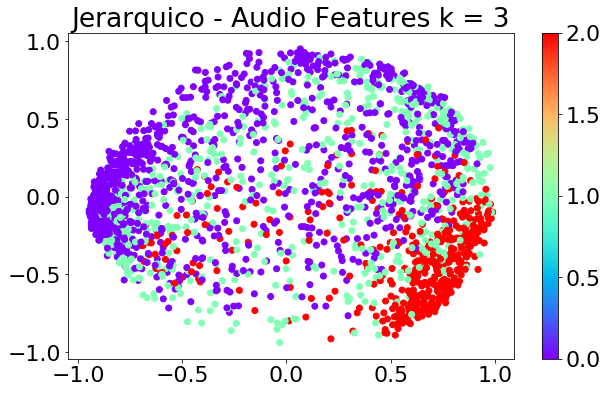
\includegraphics[width=\textwidth]{img/imagenes/jerarquico_AF/pca_3clusters.png}
    \caption{PCA}
    \label{fig:pca}
\end{figure}

Dadas las componentes 1 y 2 se observa un buen conglomerado diferenciado en especial para el cluster 2, drum-and-bass, el cual presenta su mayor densidad
en la parte positiva de la primer componente y negativa de la segunda. Lo sigue en densidad el cluster 0, y por ultimo el cluster 1 el cual presenta valores mas distribuidos y casi sin compactarse.
Cabe destactar que en el centro del grafico, proximo al valor (0,0) se pueden encontrar elementos de los 3 clusters.



\subsubsection{Audio Analisis}
Comenzamos realizando una analisis de Silhouette sobre los distintos tipos de data set $timbres\_avg$, $timbres\_std\_dev$, $pitches\_avg$ y $pitches\_std\_dev$
Para hacer esto, nos basamos en la experiencia obtenida con Audio Features, y utilizamos la misma medida Ward y la misma cantidad de clusters optimos encontrada hasta el momento de 3.

\begin{figure}[H]
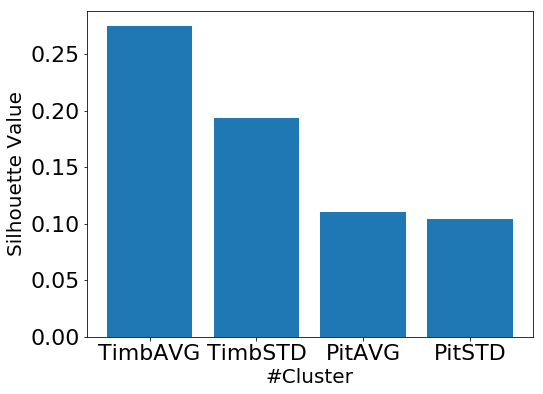
\includegraphics[width=\textwidth]{img/imagenes/jerarquico_AA/silhouette_avgstd.png}
\end{figure}
\begin{center}Comparativa general\end{center}

\begin{table}[H]
	\centering
	\begin{tabular}{ |c|c|c| }
		\hline
 		Data Set & Cantidad de clusters & Indice RAND\\
 		\hline
 		timbres avg & 3 & 0.1690\\
        timbres std & 3 & 0.0666\\
        pitches avg & 3 & 0.0754\\
        pirches std & 3 & 0.0231\\
        \hline
	\end{tabular}
     \label{tab:rand-ds}
\end{table}

Observando los valores de Silhouette, la mejor manera de clasificar a las canciones para este dataset es a traves de la media de \textbf{timbres average}.
Como proximo paso, se procede a realizar una junta entre el dataset de $audio\_features$ con $audio\_analysis$ que ya contenia el promedio de los timbres.
Para realizar un analisis mas profundo sobre este nuevo data set.

\begin{figure}[H]
    \centering
    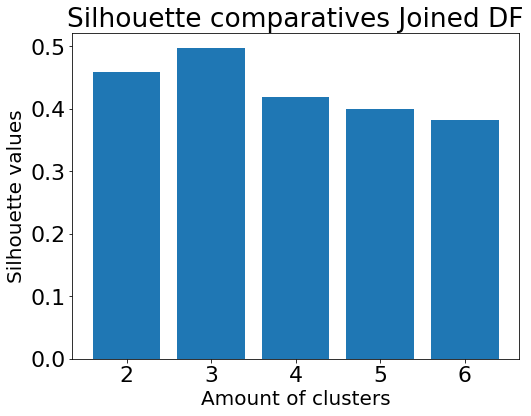
\includegraphics[width=\textwidth]{img/imagenes/jerarquico_AA/silhouette_joinedDF.png}
    \caption{Silhouette Joined DF}
    \label{fig:silJoinedDF}
\end{figure}

\begin{table}[H]
    \centering
    \begin{tabular}{|c|c|}
    	\hline
        Cantidad de clusters & Silhouette Score \\
        \hline
        2 & 0.4582\\
        3 & 0.4968\\
        4 & 0.4192\\
        5 & 0.3997\\
        6 & 0.3822\\
        \hline
    \end{tabular}
    \caption{Sil full data set}
    \label{tab:sil-fullds}
\end{table}

Nuevamente hacemos un balance entre el valor que nos arroja el Silhouette y la mejor configuracion de cantidad de K. Al igual que antes, tanto para \textbf{K=2}, \textbf{K=3}, \textbf{K=4} los valores son muy similares decidimos ir por \textbf{K=3} ya que tiene el valor mayor y ademas poder tener cierto grado de comparacion con el trabajor realizado antes.
Nos proponemos ahora a calcular los indices RAND y VanDongen

\begin{table}[H]
	\centering
	\begin{tabular}{ |c|c|c| }
		\hline
 		Cantidad de clusters & Indice RAND & Indice VanDongen\\
 		\hline
		 2 & 0.1855 & 0.6502\\
         3 & 0.3160 & 0.5194\\
         \hline
	\end{tabular}
     \label{tab:rand-ds}
\end{table}

El índice de VanDongen da un grado de pureza medio, aproximadamente un $51\%$ para el \textbf{K=3},
para el indice RAND podemos afirmar que el porcentaje de decisiones correctas del cluster es de un $31\%$, muy similar al anterior
analisis y esperable ya que estamos teniendo 3 clusters vs las 5 etiquetas que hay.

\begin{center} \textbf{Cross table} \end{center}
Para entender a mas a detalle que tan bien se realizo la clasificaciones se genera la siguiene tabla donde se aprecia el agrupamiento de generos en los dinstios clusters.

\begin{table}[H]
    \centering
    \begin{tabular}{|c|c|c|c|}
        \hline
        & \multicolumn{3}{ c| }{Clusters} \\
        \hline
        Género & 0 & 1 & 2 \\
        \hline
        ambient & 334 & 24 & 102 \\
        classical & 386 & 17 & 2 \\
        drum-and-bass & 0 & 22 & \textbf{429} \\
        jazz & 158 & 232 & 36 \\
        world-music & 93 & 334 & 36 \\  
        \hline
    \end{tabular}
    \caption{Géneros musicales y grupos full df}
    \label{tab:cross-fulldf}
\end{table}

Al revisar la conformacion de los clusters, nuevamente podemos apreciar que el genero \textbf{drum-and-bass} es quien se concentra en su mayoria
en el cluster 3.

\begin{center} \textbf{Componentes principales} \end{center}
Nuevamente realizamos un análisis de componentes principales con la finalidad de reducir la dimensionalidad del data set estudiado y asi poder lograr una representación gráfica de la division en 3 clusters.

\begin{figure}[H]
    \centering
    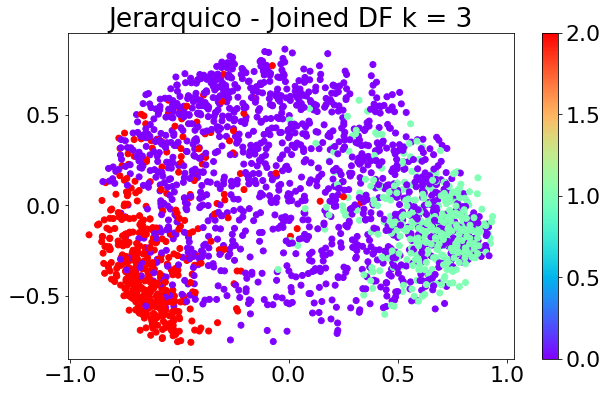
\includegraphics[width=\textwidth]{img/imagenes/jerarquico_AA/pca_joinedDF_3clusters.png}
    \caption{PCA Joined DF}
    \label{fig:pcaJoinedDF}
\end{figure}

Dadas las componentes 1 y 2 se observa un buen conglomerado diferenciado en especial para el cluster 2, drum-and-bass, el cual tiene su mayor cantidad de valores en la zona de proyeccion negativa de la primer y segunda componente. Un caso algo diferente es el del cluster 1 que si bien logra algo de aglomeración, se proyecta casi en su totalidad en la parte positiva de la primer componente e intercalando entre positivo y negativo para la segunda componente. Por ultimo esta el cluster 0, el cual muestra mayor esparcimiento y ocupando valores positivos y negativos de ambas componentes.
Se aprecia por ultimo, una separacion mas marcada entre el cluster 1 y 2, mientras que el 0 esta mas desparramado.

